\documentclass[tikz,border=8pt]{standalone}
\usepackage{tikz}
\usepackage{fontspec}
\setmainfont{DejaVu Sans}
\setsansfont{DejaVu Sans}
\usetikzlibrary{arrows.meta, positioning, shapes.geometric, calc, fit, backgrounds}
\begin{document}
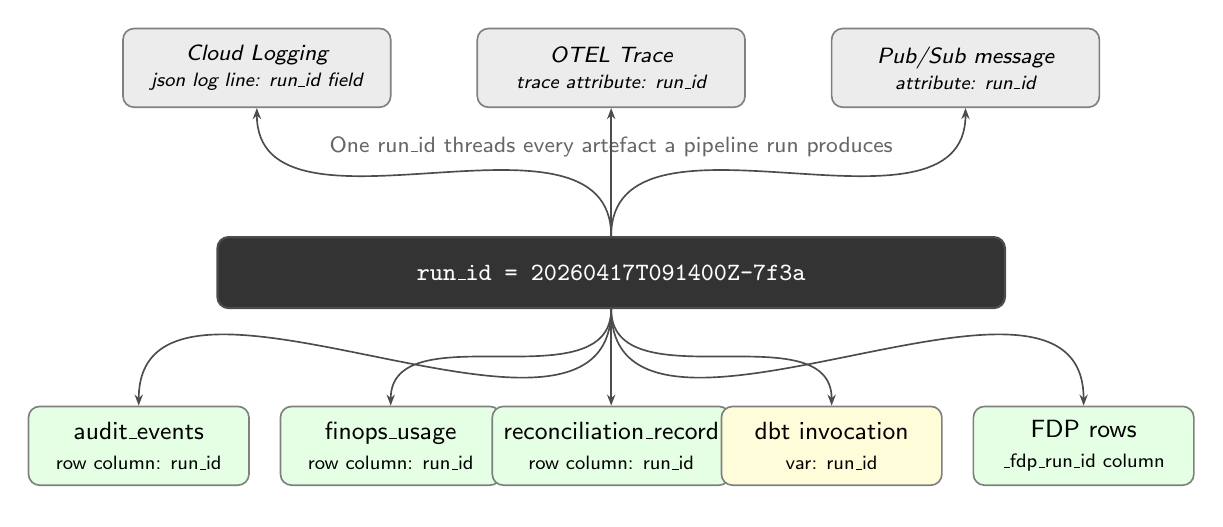
\begin{tikzpicture}[
  font=\sffamily\small,
  every node/.style={font=\sffamily\small},
  box/.style={draw=black!50, line width=0.6pt, rounded corners=4pt, minimum width=2.4cm, minimum height=1cm, align=center, inner sep=4pt},
  src/.style={box, fill=blue!10},
  storage/.style={box, fill=green!10},
  compute/.style={box, fill=yellow!15},
  output/.style={box, fill=purple!15},
  control/.style={box, fill=gray!15, font=\sffamily\footnotesize\itshape},
  err/.style={box, fill=red!10},
  arrow/.style={-{Stealth[length=4pt]}, line width=0.6pt, draw=black!70},
  dashed-arrow/.style={arrow, dashed, draw=black!50},
  caption/.style={font=\sffamily\footnotesize, text=black!60}
]

% Caption at top
\node[caption, text width=12cm, align=center] at (6, 4.8)
  {One run\_id threads every artefact a pipeline run produces};

% === CENTRAL SPINE ===
\node[draw=black!70, fill=black!80, line width=0.8pt, rounded corners=4pt,
      minimum width=10cm, minimum height=0.9cm,
      text=white, font=\sffamily\small\bfseries] (spine) at (6, 3.2)
  {\texttt{run\_id = 20260417T091400Z-7f3a}};

% === BRANCHES UP (3 boxes) ===
\node[control, minimum width=3.4cm] (clog) at (1.5, 5.8)
  {Cloud Logging\\{\scriptsize json log line: run\_id field}};
\node[control, minimum width=3.4cm] (otel) at (6.0, 5.8)
  {OTEL Trace\\{\scriptsize trace attribute: run\_id}};
\node[control, minimum width=3.4cm] (psub) at (10.5, 5.8)
  {Pub/Sub message\\{\scriptsize attribute: run\_id}};

\draw[arrow] (spine.north) to[out=90,in=-90] (clog.south);
\draw[arrow] (spine.north) -- (otel.south);
\draw[arrow] (spine.north) to[out=90,in=-90] (psub.south);

% === BRANCHES DOWN (5 boxes) ===
\node[storage, minimum width=2.8cm] (aud) at (0,   1.0)
  {audit\_events\\{\scriptsize row column: run\_id}};
\node[storage, minimum width=2.8cm] (fin) at (3.2, 1.0)
  {finops\_usage\\{\scriptsize row column: run\_id}};
\node[storage, minimum width=2.8cm] (rec) at (6.0, 1.0)
  {reconciliation\_record\\{\scriptsize row column: run\_id}};
\node[compute, minimum width=2.8cm] (dbt) at (8.8, 1.0)
  {dbt invocation\\{\scriptsize var: run\_id}};
\node[storage, minimum width=2.8cm] (fdp) at (12.0, 1.0)
  {FDP rows\\{\scriptsize \_fdp\_run\_id column}};

\draw[arrow] (spine.south) to[out=-90,in=90] (aud.north);
\draw[arrow] (spine.south) to[out=-90,in=90] (fin.north);
\draw[arrow] (spine.south) -- (rec.north);
\draw[arrow] (spine.south) to[out=-90,in=90] (dbt.north);
\draw[arrow] (spine.south) to[out=-90,in=90] (fdp.north);

\end{tikzpicture}
\end{document}
